\documentclass[conference]{IEEEtran}
\IEEEoverridecommandlockouts
\usepackage{amsmath,amssymb,amsfonts}
\usepackage{graphicx}
\usepackage{textcomp}
\usepackage{xcolor}
\usepackage{geometry}
\usepackage{booktabs}
\usepackage{array}
\usepackage[hidelinks]{hyperref}

\geometry{a4paper,left=2cm,right=2cm,top=2.5cm,bottom=4cm}
\def\BibTeX{{\rm B\kern-.05em{\sc i\kern-.025em b}\kern-.08em
    T\kern-.1667em\lower.7ex\hbox{E}\kern-.125emX}}

\newcommand{\todo}[1]{\textcolor{red}{[TODO: #1]}}
\newcommand{\method}{ArnoldiGCL-S1/S2}
\newcommand{\dti}{drug--target interaction}

\title{Leakage Safe Similarity Neighbour Side Information for Graph Based Drug Target Interaction Prediction}

\author{
    \IEEEauthorblockN{Laiyi Fu\textsuperscript{1}, Jianyu Yin\textsuperscript{2}}
    \IEEEauthorblockA{1. School of Automation Science and Engineering, Xi'an Jiaotong University, Xi'an, Shaanxi, China}
    \IEEEauthorblockA{2. Xi'an Jiaotong University, Xi'an, Shaanxi, China}
    \IEEEauthorblockA{3125354034@stu.xjtu.edu.cn}
}

\begin{document}
\maketitle

\begin{abstract}
\IfFileExists{generated/abstract_autogenerated.tex}{%
  Predicting drug--target interactions (DTIs) from molecular and protein information can prioritize candidate mechanisms, but apparent accuracy can depend on what information crosses an evaluation split. We developed ArnoldiGCL-S1/S2, a graph-based DTI predictor that combines separate drug and protein projections with seven similarity-neighbour descriptors computed only from positive training-fold interactions. Across BioSNAP, Human and BindingDB under random, cold-drug, cold-protein and cold-pair splits, the full model had the highest mean AUPR among the principal baselines in 7/12 prespecified conditions and exceeded its structural-only variant in 11/12 conditions. The latter gains ranged from 0.013 to 0.396 AUPR; 11 descriptive paired contrasts had Benjamini--Hochberg-adjusted $p<0.05$. The model was not the highest-AUPR principal baseline in BioSNAP Cold protein, Human Cold protein, Human Cold pair, BindingDB Cold protein, BindingDB Cold pair, demonstrating that the side information does not confer a uniform advantage. These results support leakage-safe similarity-neighbour summaries as a useful, but split-dependent, source of evidence for computational DTI prioritization; they do not establish prospective or experimental target binding.
%
}{%
  \todo{Write only after all fixed-fold results, effect sizes and limitations are finalized.}%
}
\end{abstract}

\begin{IEEEkeywords}
drug target interaction prediction, graph neural networks, similarity neighbours,
data leakage, cold start evaluation
\end{IEEEkeywords}

\section{Introduction}
Inferring drug--target interactions (DTIs) from molecular and protein
information can prioritize candidate mechanisms for drug discovery and
repurposing. Data-driven predictors have therefore progressed from paired
sequence or chemical representations, exemplified by DeepDTA, to graph-based
drug encoders and attention-based interaction models
\cite{ozturk2018deepdta,nguyen2021graphdta,bai2023drugban}. These approaches
have established useful representation-learning routes, but their reported
performance remains strongly coupled to what evidence is allowed to cross an
evaluation split.

This issue is particularly consequential for binary DTI prediction. A model may
perform well when a test pair contains a drug or a protein that is well
represented in the training graph, while its utility is less clear when a drug,
protein or pair is held out. Similarity between compounds or proteins can be
valuable for these settings: earlier predictors have used neighbourhood
regularization and heterogeneous network integration to incorporate related
drug and protein evidence \cite{liu2016nrlmf,luo2017dtinet}. However,
label-derived neighbour summaries must be constructed from the training
partition alone. Otherwise, a held-out DTI label can enter either message
passing or a candidate-pair feature indirectly.

Here, we study a leakage-safe use of similarity-neighbour information in a
graph-based DTI predictor. The full model, ArnoldiGCL-S1/S2, combines
separate drug and protein feature projections, a training-fold structural
encoder and seven side-information descriptors derived solely from positive
training DTIs. Rather than using similarity only as a regularizer or a network
integration mechanism, this design exposes training-fold neighbour evidence as
candidate-pair descriptors that can be ablated and shuffled. We evaluate it
against feature-only, graph-based and bilinear-attention baselines under fixed
random, cold-drug, cold-protein and cold-pair splits. The evaluation is
designed to identify not only gains from aligned neighbour information, but
also settings in which the same information does not improve over simpler
alternatives.

\section{Methods}

\subsection{Problem setting and feature representations}
We considered binary \dti{} prediction for a drug set $\mathcal{D}$ and a
protein set $\mathcal{P}$. Let $A\in\{0,1\}^{|\mathcal{D}|\times|\mathcal{P}|}$
denote the observed interaction matrix, where $A_{ij}=1$ indicates an annotated
interaction between drug $i$ and protein $j$. Each drug was represented by a
cached 1,024-bit radius-2 Morgan bit vector \cite{rogers2010ecfp}, and each protein by a cached
mean-pooled ESM-2 t30/150M embedding (640 dimensions) \cite{lin2023esm}. The drug and protein
feature encoders were distinct learnable projection networks; their parameters
were not shared.

We constructed a drug similarity matrix $S_D$ and a protein similarity matrix
$S_P$ by cosine similarity of the corresponding cached feature vectors. These
similarities were feature-derived and were not calculated from DTI labels.

\begin{figure*}[t]
\centering
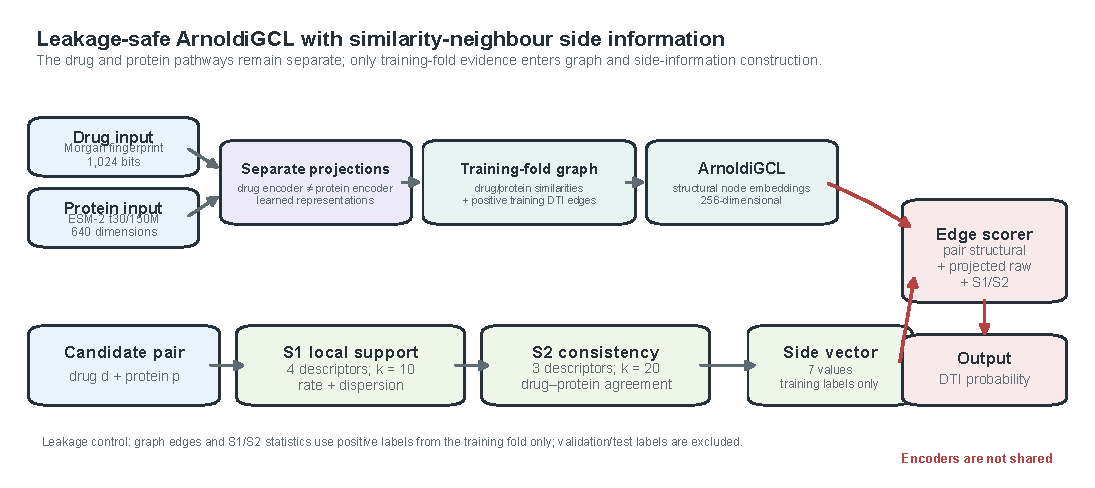
\includegraphics[width=\textwidth]{figures/figure_1_method_schematic.pdf}
\caption{Overview of the full ArnoldiGCL-S1/S2 DTI predictor. Drug Morgan
fingerprints and protein ESM-2 embeddings enter distinct learnable projection
networks; the encoder weights are not shared. A training-fold graph supplies
structural embeddings, while the S1/S2 branch derives seven candidate-pair
descriptors from feature-based neighbours and positive $A_{\mathrm{train}}$
edges only. Structural pair features, raw features and side information are
then combined by an edge scorer. Validation and test DTI labels are excluded
from graph and side-information construction.}
\label{fig:method-overview}
\end{figure*}

\subsection{Leakage-safe graph construction}
For every outer fold, the graph contained only positive DTI edges from the
training partition. Drug--drug and protein--protein similarity edges were also
restricted to entities observed in that training partition. The default graph
connected the top 10 drug neighbours and top 10 protein neighbours; all graph
edges were represented bidirectionally. The Threshold GCN baseline instead
retained within-type similarity edges whose similarity exceeded 0.3. No
validation or test DTI labels were added to a graph or side-information feature.

\subsection{ArnoldiGCL structural representation}
The projected drug and protein features were concatenated as nodes in the
training-fold graph and passed to the ArnoldiGCL encoder
\cite{coskun2025arnoldigcl}. The structural
embedding dimension was 256. The downstream edge scorer received the structural
embeddings of a candidate drug--protein pair together with the respective raw
Morgan and ESM-2 representations. The encoder was optimized for 50 epochs, and
each edge scorer was optimized for 200 epochs with Adam (learning rate
$10^{-3}$ and dropout 0.5). For encoder pretraining, the objective was binary
discrimination between the graph representation of the projected node features
and a negative view formed by a random permutation of node features. Each
update used two positive and two negative node-level logit sets, optimized with
binary cross-entropy. The drug and protein projections remained separate
throughout this objective.

\subsection{Leakage-safe S1/S2 side information}
For a candidate pair $(i,j)$, all side information was computed from the binary
matrix $A_{\mathrm{train}}$ that contains positive training DTI edges only. Let
$N_D^k(i)$ and $N_P^k(j)$ be the top-$k$ most similar training drugs and
proteins, respectively. A queried entity was excluded from its own
neighbourhood.

The S1 module used $k=10$ and produced four descriptors: the mean and standard
deviation of $A_{d,j}$ over $d\in N_D^{10}(i)$, and the mean and standard
deviation of $A_{d,p}$ over $d\in N_D^{10}(i), p\in N_P^{10}(j)$. Thus, S1
summarizes local neighbour support and its dispersion without accessing the
label of the candidate pair.

The S2 module used $k=20$ and produced three consistency descriptors: the mean
of $A_{d,j}$ over $d\in N_D^{20}(i)$, the mean of $A_{i,p}$ over
$p\in N_P^{20}(j)$, and the mean of $A_{d,p}$ over the corresponding drug and
protein neighbour cross-product. The seven S1/S2 values were passed through the
side-information branch of the edge scorer. The S1-only and S2-only ablations
zero-padded the complementary descriptors; the shuffled control permuted the
seven-dimensional side-information vectors within each partition while
preserving their marginal distribution.

\subsection{Comparators and implementation details}
The benchmark includes logistic regression and an MLP on concatenated Morgan
and ESM-2 representations, a two-layer GCN on the leak-safe $k$NN graph, a
Threshold GCN comparator, and DrugBAN
\cite{ozturk2018deepdta,nguyen2021graphdta,bai2023drugban}. All compared methods
use the same frozen positive partitions and partition-specific negative
examples. This aligns the evaluated drug--protein pairs across methods but
does not force identical input modalities: DrugBAN consumes canonical
SMILES-derived graphs and protein sequences, whereas the feature and graph
comparators use the frozen Morgan and ESM-2 representations described above.
DrugBAN is consequently reported as a matched-partition comparator in this
benchmark, not as a claim to reproduce its published benchmark scores.
For DrugBAN, deterministic SMILES-to-graph and protein integer
preprocessing was cached within a fold when an input recurred; this does not
alter the DrugBAN architecture, optimizer or emitted batch values. DrugBAN was
trained with Adam at a learning rate of $5\times10^{-5}$, batch size 64 and a
fixed 100-epoch schedule; the validation-AUC checkpoint was evaluated once on
the corresponding test partition. All DrugBAN folds used TensorFloat-32 matrix
operations on NVIDIA GeForce RTX 4080 SUPER GPUs; this execution setting was
recorded in every
result artifact and held fixed across B5 folds.
The two GCN baselines use cached sparse normalized aggregation on BindingDB to
bound peak memory. This implementation was verified against the original dense
aggregation for forward output and backward gradients, and was smoke-tested on
the full BindingDB threshold graph before running the queue.

\section{Experimental protocol}

\subsection{Datasets and frozen evaluation splits}
We evaluate BioSNAP, Human and BindingDB under four scenarios: random,
cold-drug, cold-protein and cold-pair splits. Each scenario uses three fixed
random seeds and five outer folds, yielding 15 held-out evaluations per
dataset--scenario--method combination. Within each outer training partition,
approximately 10\% of eligible training positives are reserved for model
selection. For cold-drug and cold-protein splits, validation and test entities
are disjoint from training entities. For cold-pair splits, train, validation
and test positives are sampled from disjoint diagonal drug--protein blocks;
off-block pairs are not evaluated.

The three local \texttt{full.csv} files were verified as exact Git-blob matches
to the pinned DrugBAN dataset snapshot (commit
\texttt{9923f8c99959e00263103ff9ac61ba0eaccc8e02}). Its dataset documentation
identifies BindingDB, BioSNAP as distributed by MolTrans, and Human as
distributed by TransformerCPI \cite{bai2023drugban,liu2007bindingdb,huang2021moltrans,chen2020transformercpi}.
The generated dataset manifest records this source snapshot, byte-level
checksums and the observed input schema for every run.

For every partition, up to 10 unique unannotated pairs were sampled per
positive without replacement. Test and validation negatives were allocated
before training negatives to make held-out samples invariant to later
training-set changes. In unusually dense blocks with fewer available unique
negatives, all available unique negatives were used and the realized partition
size was retained in the fold-level result record.

\subsection{Realized benchmark coverage}
The completed release contains 180 frozen split definitions and 1,800
formal result records. This corresponds to 3 datasets, 4 split scenarios,
10 model variants and 15 seed--fold evaluations for every
dataset--scenario--method combination. All expected records passed the
release audit, and no dataset--scenario--method group had missing folds.
The realized test-set sizes were $30,426 \pm 0$ pairs for BioSNAP Random,
$5,793 \pm 6$ pairs for Human Random and $45,483 \pm 5$ pairs for
BindingDB Random. Under cold-pair evaluation, the corresponding test-set
sizes were $6,173 \pm 864$, $1,168 \pm 411$ and $9,107 \pm 1,732$ pairs,
respectively. The larger variation in the cold-start settings reflects the
number of eligible entities and unannotated drug--protein pairs available
within each frozen partition.

Across the complete benchmark, the mean number of test positives per fold
was $2,766 \pm 0$ for BioSNAP Random, $527 \pm 1$ for Human Random and
$4,135 \pm 0$ for BindingDB Random. In the cold-pair setting, the
corresponding values were $561 \pm 79$, $106 \pm 37$ and $828 \pm 157$.
These realized counts, together with the train and validation counts for
every dataset and split, are provided in Table~\ref{tab:fold-sizes} and in
the accompanying fold-level source-data CSV.

\subsection{Comparator families}
Table~\ref{tab:comparators} distinguishes feature-only, graph-based,
bilinear-attention and ablation controls. All rows use exactly the same frozen
positive partitions and partition-specific negative examples. ``Threshold GCN''
is a comparator implemented with the specified 0.3 within-type similarity
threshold; it is not presented as a full reproduction of an external method.
The panel is intended for controlled matched-partition comparisons rather than
an exhaustive reproduction of every published DTI method; conclusions are
therefore restricted to this benchmark.

\begin{table*}[t]
\centering
\scriptsize
\begin{tabular}{p{0.16\textwidth}p{0.22\textwidth}p{0.54\textwidth}}
\toprule
Family & Model & Information available to the model \\
\midrule
Feature-only & Logistic regression & Concatenated Morgan and ESM-2 pair features. \\
Feature-only & MLP & Concatenated Morgan and ESM-2 pair features. \\
Graph-based & GCN & Fold-local positive DTI graph with top-10 within-type similarity neighbours. \\
Graph-based & Threshold GCN & Fold-local positive DTI graph with within-type similarity edges above 0.3. \\
Bilinear-attention & DrugBAN & Canonical molecular graph and protein-sequence inputs, trained on the same frozen pair partitions. \\
Ablation & ArnoldiGCL w/o S1/S2; +S1; +S2; shuffled S1/S2 & The same fold-local ArnoldiGCL structural encoder, with the indicated side-information treatment. \\
Full model & ArnoldiGCL-S1/S2 & Structural pair features, raw Morgan and ESM-2 features, and aligned seven-dimensional S1/S2 information. \\
\bottomrule
\end{tabular}
\caption{Prespecified comparator families. All learning, graph construction
and label-derived side information are restricted to the outer training fold.}
\label{tab:comparators}
\end{table*}

\subsection{Evaluation and statistical reporting}
We report area under the receiver operating characteristic curve (AUC), area
under the precision--recall curve (AUPR), F1 score and accuracy. Checkpoints
were selected by validation AUC; F1 thresholds were selected by maximal
validation F1 and applied once to the test partition. The primary tables will
report mean $\pm$ sample standard deviation across 15 fixed seed--fold
evaluations. Pairwise comparisons will be paired by identical seed--fold
identity and summarized with effect sizes and two-sided Wilcoxon signed-rank
statistics. Because folds sharing a random seed are not independent biological
or experimental replicates, these $p$-values are descriptive summaries of
paired fold differences rather than confirmatory population-level inference.
For the complete family of reported descriptive comparisons, two-sided
$p$-values will be adjusted using the Benjamini--Hochberg procedure; both raw
and adjusted values will be provided as source data.

\subsection{Ablation and robustness analyses}
We compare the full S1/S2 model with a structural-only version, S1-only and
S2-only variants, and a partition-wise shuffled S1/S2 control. The shuffled
control distinguishes the presence of extra numerical inputs from alignment
between side information and the evaluated drug--protein pair.

\IfFileExists{generated/protocol_autogenerated.tex}{%
  \subsection{Fold-level dataset sizes}
Table~\ref{tab:fold-sizes} reports realized sample counts across the frozen folds. Counts may vary across cold-start folds because entities and eligible unannotated pairs are partition-specific.
\begin{table*}[t]
\centering
\scriptsize
\begin{tabular}{llrrrr}
\toprule
Dataset & Split & Train pairs & Validation pairs & Test pairs & Test positives \\
\midrule
BioSNAP & Random & 109538 $\pm$ 0 & 12166 $\pm$ 0 & 30426 $\pm$ 0 & 2766 $\pm$ 0 \\
BioSNAP & Cold drug & 109724 $\pm$ 1569 & 11980 $\pm$ 750 & 30426 $\pm$ 1336 & 2766 $\pm$ 121 \\
BioSNAP & Cold protein & 109120 $\pm$ 4026 & 12584 $\pm$ 3126 & 30426 $\pm$ 3839 & 2766 $\pm$ 349 \\
BioSNAP & Cold pair & 78327 $\pm$ 3469 & 1021 $\pm$ 315 & 6173 $\pm$ 864 & 561 $\pm$ 79 \\
\midrule
Human & Random & 20849 $\pm$ 6 & 2321 $\pm$ 0 & 5793 $\pm$ 6 & 527 $\pm$ 1 \\
Human & Cold drug & 21054 $\pm$ 989 & 2116 $\pm$ 912 & 5793 $\pm$ 1194 & 527 $\pm$ 109 \\
Human & Cold protein & 20789 $\pm$ 1099 & 2382 $\pm$ 843 & 5793 $\pm$ 1139 & 527 $\pm$ 104 \\
Human & Cold pair & 15101 $\pm$ 1453 & 150 $\pm$ 112 & 1168 $\pm$ 411 & 106 $\pm$ 37 \\
\midrule
BindingDB & Random & 163737 $\pm$ 5 & 18194 $\pm$ 0 & 45483 $\pm$ 5 & 4135 $\pm$ 0 \\
BindingDB & Cold drug & 163701 $\pm$ 700 & 18230 $\pm$ 466 & 45483 $\pm$ 685 & 4135 $\pm$ 62 \\
BindingDB & Cold protein & 163327 $\pm$ 8143 & 18605 $\pm$ 4576 & 45483 $\pm$ 8652 & 4135 $\pm$ 787 \\
BindingDB & Cold pair & 118036 $\pm$ 8799 & 1481 $\pm$ 538 & 9107 $\pm$ 1732 & 828 $\pm$ 157 \\
\bottomrule
\end{tabular}
\caption{Realized fold sizes (mean $\pm$ sample standard deviation across 15 fixed seed--fold evaluations).}
\label{tab:fold-sizes}
\end{table*}
%
}{%
  \todo{Insert final dataset statistics from the completed artifacts.}%
}

\subsection{Compute environment and reproducibility}
The principal benchmark was executed on NVIDIA GeForce RTX 4080 SUPER GPUs. Every
result artifact records the dataset, scenario, seed, outer fold, split
signature, validation criterion, test metrics and realized partition sizes.
DrugBAN artifacts additionally record the fixed 100-epoch schedule, input
preprocessing cache and TensorFloat-32 setting. The release-time environment
manifest records the software versions, GPU/driver information and hashes of
the key benchmark scripts. Aggregate wall-clock time is not reported because
per-fold duration is not a standardized field in every result artifact.

\section{Results}

\subsection{Complete benchmark comparison}

Tables~\ref{tab:benchmark-aupr} and \ref{tab:benchmark-auc} report test performance from the complete frozen-fold benchmark. The accompanying source-data CSV records every seed--fold value and the paired-comparison file contains raw and Benjamini--Hochberg-adjusted Wilcoxon $p$-values.

\begin{figure*}[t]
\centering
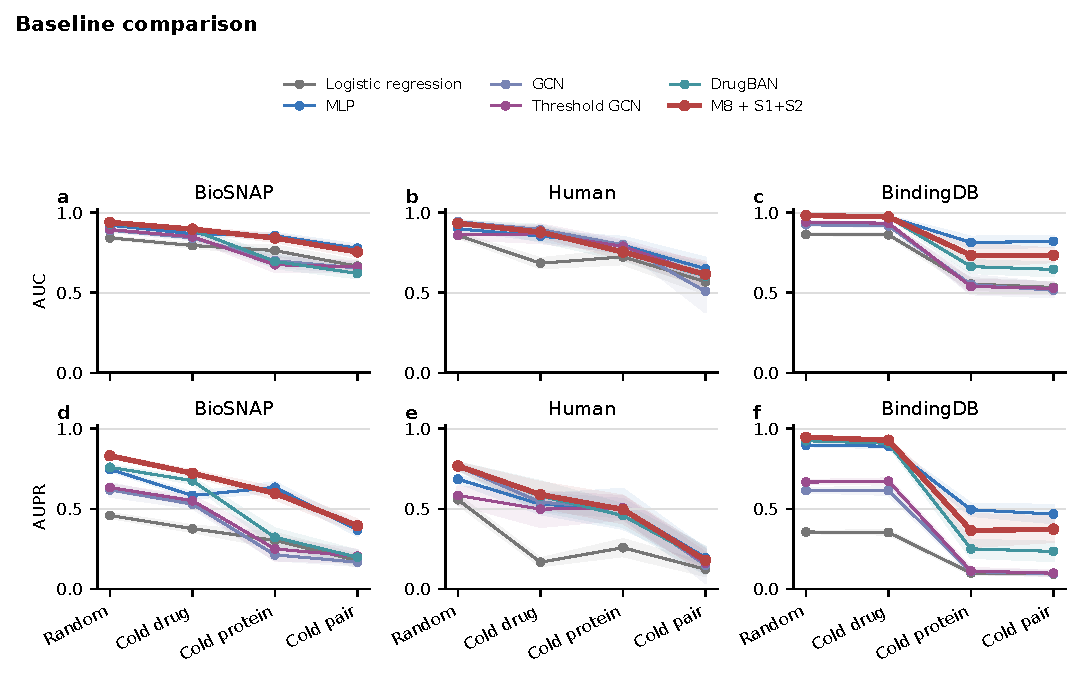
\includegraphics[width=\textwidth]{figures/figure_2_baselines.pdf}
\caption{Comparison of feature-only, graph-based, bilinear-attention and full S1/S2 models across the four fixed split scenarios. Each point is the mean of 15 seed--fold evaluations and the shaded band denotes the sample standard deviation.}
\label{fig:baseline-comparison}
\end{figure*}

Across the 12 prespecified dataset--split conditions, ArnoldiGCL-S1/S2 had the highest mean AUPR among the principal baselines in 7/12 conditions. The conditions without the highest mean AUPR were BioSNAP Cold protein, Human Cold protein, Human Cold pair, BindingDB Cold protein, BindingDB Cold pair.

\begin{table*}[t]
\centering
\scriptsize
\resizebox{\textwidth}{!}{%
\begin{tabular}{llcccccc}
\toprule
Dataset & Split & Logistic regression & MLP & GCN & Threshold GCN & DrugBAN & M8 + S1+S2 \\
\midrule
BioSNAP & Random & 0.458 $\pm$ 0.012 & 0.746 $\pm$ 0.008 & 0.618 $\pm$ 0.039 & 0.633 $\pm$ 0.016 & 0.759 $\pm$ 0.010 & 0.831 $\pm$ 0.007 \\
BioSNAP & Cold drug & 0.376 $\pm$ 0.019 & 0.583 $\pm$ 0.017 & 0.529 $\pm$ 0.022 & 0.551 $\pm$ 0.025 & 0.675 $\pm$ 0.017 & 0.722 $\pm$ 0.015 \\
BioSNAP & Cold protein & 0.303 $\pm$ 0.044 & 0.634 $\pm$ 0.030 & 0.212 $\pm$ 0.031 & 0.250 $\pm$ 0.070 & 0.322 $\pm$ 0.052 & 0.597 $\pm$ 0.034 \\
BioSNAP & Cold pair & 0.177 $\pm$ 0.034 & 0.367 $\pm$ 0.034 & 0.166 $\pm$ 0.021 & 0.203 $\pm$ 0.037 & 0.197 $\pm$ 0.039 & 0.394 $\pm$ 0.036 \\
\midrule
Human & Random & 0.557 $\pm$ 0.027 & 0.685 $\pm$ 0.019 & 0.765 $\pm$ 0.018 & 0.584 $\pm$ 0.054 & 0.766 $\pm$ 0.021 & 0.768 $\pm$ 0.018 \\
Human & Cold drug & 0.166 $\pm$ 0.022 & 0.529 $\pm$ 0.059 & 0.541 $\pm$ 0.052 & 0.498 $\pm$ 0.109 & 0.579 $\pm$ 0.091 & 0.588 $\pm$ 0.075 \\
Human & Cold protein & 0.257 $\pm$ 0.050 & 0.500 $\pm$ 0.123 & 0.503 $\pm$ 0.055 & 0.506 $\pm$ 0.070 & 0.458 $\pm$ 0.067 & 0.496 $\pm$ 0.083 \\
Human & Cold pair & 0.122 $\pm$ 0.039 & 0.195 $\pm$ 0.052 & 0.149 $\pm$ 0.107 & 0.160 $\pm$ 0.062 & 0.177 $\pm$ 0.084 & 0.178 $\pm$ 0.065 \\
\midrule
BindingDB & Random & 0.355 $\pm$ 0.004 & 0.897 $\pm$ 0.003 & 0.615 $\pm$ 0.010 & 0.667 $\pm$ 0.010 & 0.925 $\pm$ 0.004 & 0.947 $\pm$ 0.003 \\
BindingDB & Cold drug & 0.352 $\pm$ 0.011 & 0.891 $\pm$ 0.010 & 0.614 $\pm$ 0.024 & 0.673 $\pm$ 0.014 & 0.909 $\pm$ 0.010 & 0.928 $\pm$ 0.007 \\
BindingDB & Cold protein & 0.099 $\pm$ 0.009 & 0.494 $\pm$ 0.036 & 0.108 $\pm$ 0.010 & 0.111 $\pm$ 0.016 & 0.250 $\pm$ 0.053 & 0.364 $\pm$ 0.100 \\
BindingDB & Cold pair & 0.093 $\pm$ 0.006 & 0.467 $\pm$ 0.054 & 0.095 $\pm$ 0.015 & 0.098 $\pm$ 0.013 & 0.234 $\pm$ 0.058 & 0.373 $\pm$ 0.077 \\
\bottomrule
\end{tabular}%
}
\caption{Test AUPR for the principal baseline comparison. Values are mean $\pm$ sample standard deviation across 15 fixed seed--fold evaluations.}
\label{tab:benchmark-aupr}
\end{table*}

\begin{table*}[t]
\centering
\scriptsize
\resizebox{\textwidth}{!}{%
\begin{tabular}{llcccccc}
\toprule
Dataset & Split & Logistic regression & MLP & GCN & Threshold GCN & DrugBAN & M8 + S1+S2 \\
\midrule
BioSNAP & Random & 0.842 $\pm$ 0.005 & 0.922 $\pm$ 0.005 & 0.890 $\pm$ 0.008 & 0.894 $\pm$ 0.006 & 0.930 $\pm$ 0.003 & 0.939 $\pm$ 0.004 \\
BioSNAP & Cold drug & 0.795 $\pm$ 0.011 & 0.868 $\pm$ 0.008 & 0.842 $\pm$ 0.013 & 0.850 $\pm$ 0.013 & 0.892 $\pm$ 0.008 & 0.897 $\pm$ 0.008 \\
BioSNAP & Cold protein & 0.763 $\pm$ 0.028 & 0.856 $\pm$ 0.015 & 0.700 $\pm$ 0.036 & 0.675 $\pm$ 0.043 & 0.696 $\pm$ 0.040 & 0.841 $\pm$ 0.022 \\
BioSNAP & Cold pair & 0.665 $\pm$ 0.032 & 0.777 $\pm$ 0.021 & 0.654 $\pm$ 0.027 & 0.661 $\pm$ 0.032 & 0.620 $\pm$ 0.027 & 0.755 $\pm$ 0.028 \\
\midrule
Human & Random & 0.858 $\pm$ 0.012 & 0.899 $\pm$ 0.009 & 0.944 $\pm$ 0.007 & 0.860 $\pm$ 0.023 & 0.939 $\pm$ 0.008 & 0.934 $\pm$ 0.006 \\
Human & Cold drug & 0.684 $\pm$ 0.028 & 0.854 $\pm$ 0.027 & 0.894 $\pm$ 0.014 & 0.868 $\pm$ 0.056 & 0.871 $\pm$ 0.050 & 0.878 $\pm$ 0.025 \\
Human & Cold protein & 0.724 $\pm$ 0.043 & 0.796 $\pm$ 0.050 & 0.799 $\pm$ 0.018 & 0.789 $\pm$ 0.036 & 0.751 $\pm$ 0.045 & 0.755 $\pm$ 0.043 \\
Human & Cold pair & 0.569 $\pm$ 0.072 & 0.650 $\pm$ 0.067 & 0.508 $\pm$ 0.128 & 0.610 $\pm$ 0.069 & 0.604 $\pm$ 0.067 & 0.614 $\pm$ 0.077 \\
\midrule
BindingDB & Random & 0.865 $\pm$ 0.002 & 0.978 $\pm$ 0.001 & 0.924 $\pm$ 0.002 & 0.941 $\pm$ 0.002 & 0.979 $\pm$ 0.002 & 0.982 $\pm$ 0.001 \\
BindingDB & Cold drug & 0.861 $\pm$ 0.005 & 0.973 $\pm$ 0.004 & 0.917 $\pm$ 0.005 & 0.934 $\pm$ 0.005 & 0.973 $\pm$ 0.004 & 0.973 $\pm$ 0.003 \\
BindingDB & Cold protein & 0.554 $\pm$ 0.034 & 0.814 $\pm$ 0.034 & 0.551 $\pm$ 0.058 & 0.539 $\pm$ 0.040 & 0.663 $\pm$ 0.037 & 0.734 $\pm$ 0.071 \\
BindingDB & Cold pair & 0.533 $\pm$ 0.028 & 0.820 $\pm$ 0.032 & 0.515 $\pm$ 0.041 & 0.527 $\pm$ 0.035 & 0.645 $\pm$ 0.040 & 0.734 $\pm$ 0.039 \\
\bottomrule
\end{tabular}%
}
\caption{Test AUC for the principal baseline comparison. Values are mean $\pm$ sample standard deviation across 15 fixed seed--fold evaluations.}
\label{tab:benchmark-auc}
\end{table*}

\subsection{Contribution of S1 and S2}

Table~\ref{tab:ablation-aupr} reports the prespecified structural-only, single-module and shuffled controls. Relative to the structural-only variant, the full S1/S2 model had higher mean AUPR in 11/12 conditions; among these, 11 had a descriptive paired Wilcoxon contrast with BH-adjusted $p<0.05$. The positive mean differences ranged from 0.013 to 0.396. The full model was not higher than the structural-only variant in Human Cold pair.

\begin{figure*}[t]
\centering
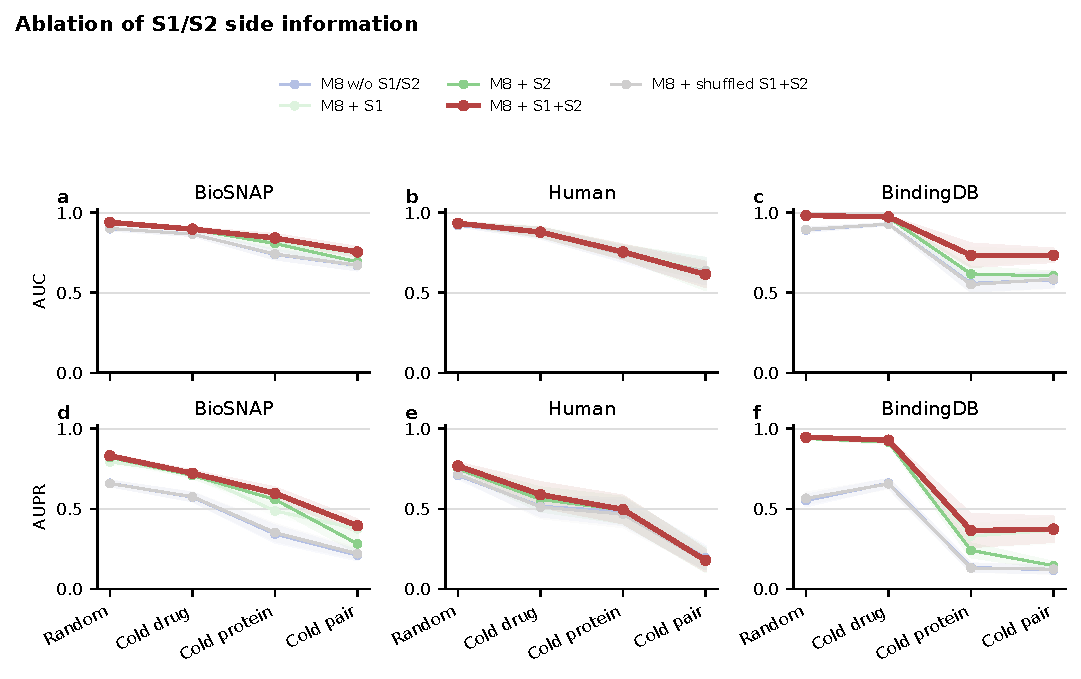
\includegraphics[width=\textwidth]{figures/figure_3_ablation.pdf}
\caption{Ablation of S1/S2 side information. The shuffled control preserves the marginal values of the seven descriptors within each partition but disrupts their association with candidate drug--protein pairs. Each point is the mean of 15 seed--fold evaluations and the shaded band denotes the sample standard deviation.}
\label{fig:side-information-ablation}
\end{figure*}

\begin{table*}[t]
\centering
\scriptsize
\resizebox{\textwidth}{!}{%
\begin{tabular}{llccccc}
\toprule
Dataset & Split & M8 w/o S1/S2 & M8 + S1 & M8 + S2 & M8 + S1+S2 & M8 + shuffled S1+S2 \\
\midrule
BioSNAP & Random & 0.659 $\pm$ 0.015 & 0.793 $\pm$ 0.008 & 0.821 $\pm$ 0.008 & 0.831 $\pm$ 0.007 & 0.658 $\pm$ 0.014 \\
BioSNAP & Cold drug & 0.573 $\pm$ 0.024 & 0.721 $\pm$ 0.017 & 0.708 $\pm$ 0.014 & 0.722 $\pm$ 0.015 & 0.575 $\pm$ 0.024 \\
BioSNAP & Cold protein & 0.342 $\pm$ 0.050 & 0.487 $\pm$ 0.027 & 0.558 $\pm$ 0.049 & 0.597 $\pm$ 0.034 & 0.352 $\pm$ 0.051 \\
BioSNAP & Cold pair & 0.210 $\pm$ 0.029 & 0.375 $\pm$ 0.047 & 0.281 $\pm$ 0.052 & 0.394 $\pm$ 0.036 & 0.220 $\pm$ 0.029 \\
\midrule
Human & Random & 0.709 $\pm$ 0.019 & 0.766 $\pm$ 0.015 & 0.749 $\pm$ 0.020 & 0.768 $\pm$ 0.018 & 0.716 $\pm$ 0.017 \\
Human & Cold drug & 0.516 $\pm$ 0.060 & 0.589 $\pm$ 0.072 & 0.558 $\pm$ 0.072 & 0.588 $\pm$ 0.075 & 0.511 $\pm$ 0.066 \\
Human & Cold protein & 0.482 $\pm$ 0.081 & 0.492 $\pm$ 0.088 & 0.492 $\pm$ 0.079 & 0.496 $\pm$ 0.083 & 0.467 $\pm$ 0.079 \\
Human & Cold pair & 0.195 $\pm$ 0.070 & 0.184 $\pm$ 0.058 & 0.180 $\pm$ 0.072 & 0.178 $\pm$ 0.065 & 0.172 $\pm$ 0.047 \\
\midrule
BindingDB & Random & 0.551 $\pm$ 0.033 & 0.941 $\pm$ 0.004 & 0.939 $\pm$ 0.004 & 0.947 $\pm$ 0.003 & 0.565 $\pm$ 0.033 \\
BindingDB & Cold drug & 0.660 $\pm$ 0.023 & 0.928 $\pm$ 0.006 & 0.916 $\pm$ 0.008 & 0.928 $\pm$ 0.007 & 0.656 $\pm$ 0.026 \\
BindingDB & Cold protein & 0.134 $\pm$ 0.023 & 0.330 $\pm$ 0.070 & 0.240 $\pm$ 0.040 & 0.364 $\pm$ 0.100 & 0.130 $\pm$ 0.021 \\
BindingDB & Cold pair & 0.118 $\pm$ 0.019 & 0.365 $\pm$ 0.078 & 0.145 $\pm$ 0.021 & 0.373 $\pm$ 0.077 & 0.123 $\pm$ 0.026 \\
\bottomrule
\end{tabular}%
}
\caption{Test AUPR for the S1/S2 ablations and shuffled control. Values are mean $\pm$ sample standard deviation across 15 fixed seed--fold evaluations.}
\label{tab:ablation-aupr}
\end{table*}

\subsection{Where the method does not improve}

The complete source data, rather than a selected subset of splits, are used for all comparative statements. In particular, the principal-baseline comparison did not place the full model first in BioSNAP Cold protein, Human Cold protein, Human Cold pair, BindingDB Cold protein, BindingDB Cold pair. These settings are retained in the figures, tables and Discussion rather than being omitted from the main comparison.



\IfFileExists{generated/discussion_autogenerated.tex}{%
  \section{Discussion}

The fixed-fold benchmark indicates that similarity-neighbour information can add predictive signal beyond the training-fold structural encoder, but only when its construction is constrained to the training partition. The full S1/S2 model had higher mean AUPR than the structural-only variant in 11/12 conditions, and 11 descriptive paired contrasts had a Benjamini--Hochberg-adjusted $p<0.05$. This pattern is consistent with the interpretation that local neighbourhood support and drug--protein consistency can complement graph-derived pair representations.

The shuffled control provides a narrower interpretation of this association. The full model had higher mean AUPR than the shuffled S1/S2 control in 12/12 conditions, including 11 descriptive paired contrasts with FDR-adjusted $p<0.05$. Because shuffling preserves the marginal side-feature values while breaking their alignment with each candidate pair, the comparison suggests that aligned side information, rather than only feature scale or dimensionality, contributes to the observed differences. It does not by itself establish a biological mechanism for any predicted interaction.

The result is not a claim of uniform superiority. The full model was not the highest-AUPR principal baseline in BioSNAP Cold protein, Human Cold protein, Human Cold pair, BindingDB Cold protein, BindingDB Cold pair. These settings should be treated as part of the method boundary: a similarity-neighbour summary may be less informative when representation coverage, dataset composition or the held-out entity structure differs from the conditions in which it is advantageous.

Several limitations follow directly from the evaluation design. The labels are curated DTIs, and the capped samples of unannotated pairs may include unknown positives; the reported metrics therefore describe the specified benchmark sampling distributions rather than the prevalence of interactions in a complete chemical--proteomic space. The study uses fixed molecular and protein feature caches, rather than learning representations from raw structures or sequences within each fold. Finally, the benchmark evaluates ranking and classification against annotated labels; experimental binding assays and prospective candidate selection are required before a prediction can support a pharmacological claim.
%
}{%
  \section{Discussion}
  \todo{Interpret the complete benchmark, including scenarios with no gain over simpler baselines.}%
}

\IfFileExists{generated/conclusion_autogenerated.tex}{%
  \section{Conclusion}

ArnoldiGCL-S1/S2 integrates separate drug and protein projections, a training-fold graph encoder and leakage-safe S1/S2 similarity-neighbour descriptors for DTI prediction. Under the complete fixed-fold benchmark, the full model exceeded its structural-only counterpart in 11/12 AUPR comparisons and was the highest-AUPR principal baseline in 7/12 conditions. The evidence supports the use of fold-local neighbour information as a split-dependent computational prioritization signal, while preserving the observed non-winning settings and the need for prospective experimental validation.
%
}{}

\section{Data and code availability}

\noindent\textbf{Generated benchmark artifacts.} The frozen train, validation
and test partitions, per-fold result JSON files, aggregate tables, figure source
data and the dataset manifest generated in this study will be deposited in
\todo{repository name and persistent identifier} before publication. The
manifest records the SHA256 checksum, Git-blob checksum, observed schema and
pinned upstream snapshot of every input CSV used for the benchmark.

\noindent\textbf{Reused input data.} The benchmark uses local CSV files labelled
BioSNAP, Human and BindingDB. Each file was verified byte-for-byte against the
corresponding \texttt{full.csv} file in the DrugBAN repository dataset snapshot
(commit \texttt{9923f8c99959e00263103ff9ac61ba0eaccc8e02}); that snapshot
documents BindingDB, MolTrans/BioSNAP and TransformerCPI/Human as the respective
sources \cite{bai2023drugban,liu2007bindingdb,huang2021moltrans,chen2020transformercpi}.
The DrugBAN repository is MIT-licensed; original data-provider terms govern
reuse and redistribution, so this manuscript does not claim that the local
copies may be redistributed.

\noindent\textbf{Code availability.} The frozen split generator, benchmark
runners, plotting scripts, manuscript generators and final audit script will be
made available at \todo{code repository and commit or release tag}. The release
will include environment specifications and commands required to regenerate the
reported tables and figures from the archived result artifacts.


\section*{Acknowledgment}
The authors thank the maintainers of the public datasets and software used in
this study.

\section*{Declarations}
\noindent\textbf{Author contributions.} Laiyi Fu conducted the study and
prepared the manuscript. Jianyu Yin contributed to the methodology and
manuscript review.

\noindent\textbf{Competing interests.} The authors declare no competing interests.

\bibliographystyle{unsrt}
\bibliography{references}
\end{document}
